\section{Korekcia optima nominálneho modelu}
V tomto okamihu už máme pripravené dátové modely, ktoré môžeme použiť na úpravu nominálneho modelu štýlom ako uvádza rovnica \ref{eq:hybrid_opt_bio} resp. \ref{eq:hybrid_opt_subs}. Než si však ukážeme výsledky prístupu využitím hybridných modelov, poďme sa pozrieť, ako dokážu problematiku optimalizácie zariadenia s nesprávnym mechanickým modelom vyriešiť spomínané dva prístupy -- dvojkroková optimalizácia a schéma úpravy modifikátora. Výsledky potom porovnáme s hybridnými modelmi. 

\subsection{Dvojkroková optimalizácia}
V teoretickej časti sme spomenuli, že k odhadu parametrov nominálneho modelu môžeme pristupovať dvojako a na základe dát, ktoré máme k dispozícii. Aproximácia derivácie nutne potrebuje údaje o koncentrácii ako biomasy tak aj substrátu, presne ako uvádza rovnica \eqref{eq:twostep_der_app}. Výsledky takéhoto odhadu parametrov môžeme vidieť na Obr. \ref{fig:twostep_derApp_pe}. Tento obrázok zobrazuje priebeh koncentrácie substrátu nominálneho modelu (modrá) na základe nameraných údajov zo zariadenia (čierna) a tak isto priebeh zo zariadenia bez vplyvu šumu (červená) pri viacerých skokových zmenách. Ako môžeme pozorovať, tak takýto prístup k odhadu parametrov dokáže celkom dobre aproximovať dynamiku systému, ale v odhade ustálených stavov sú nedostatky. Pri aproximácii derivácie sú dva faktory, ktoré nám v tomto prípade môžu ovplyvniť samotný výsledok. V prvom rade je to šum merania, ktorý svojou vlastnou dynamikou
% RP: "prehlušuje" je prilis neformalne
prehlušuje dynamiku systému. V druhom rade ide o samotnú periódu vzorkovania. Je jasné, že spätná diferencia bude zodpovedať derivácii práve vtedy, ak sa perióda vzorkovania bude limitne blížiť k nule a to nedokážeme dosiahnuť pri biochemickom reaktore. V reálnom zariadení by sme koncentráciu substrátu teoreticky vedeli merať častejšie, problematické je však meranie koncentrácie biomasy, ktorá sa bežne ani nemeria. Z tohto dôvodu sme demonštrovali ďalší prístup k odhadu parametrov, ktorý využíva iba údaje o koncentrácii substrátu a na základe týchto dát odhaduje parametre modelu tak ako uvádza rovnica \eqref{eq:twostep_diff_pe}. Takýto prístup je výrazne lepší a dokáže  odhadnúť neznáme parametre nominálneho modelu, ktorý sa nezhoduje so zariadením, tak, aby identifikovaný model dokázal opísať skutočnosť, ako zobrazuje Obr. \ref{fig:twostep_diff_pe}. Jasnou výhodou je, že koncentráciu substrátu dokážeme merať častejšie a s menšou fluktuáciou ako v prípade biomasy. 
\begin{figure}
	\centering
	\begin{subfigure}[b]{0.49\textwidth}
		\centering\
		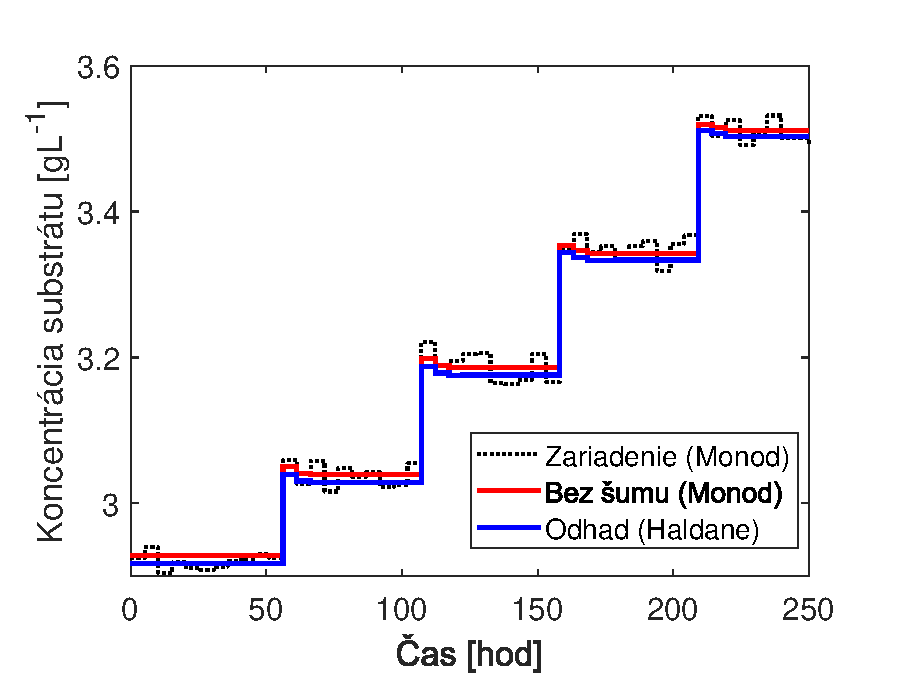
\includegraphics[width=\linewidth]{images/TwoStep_der_app_sub}
		\caption{Aproximácia derivácie.}
		\label{fig:twostep_derApp_pe}
	\end{subfigure}
	\begin{subfigure}[b]{0.49\textwidth}
		\centering\
		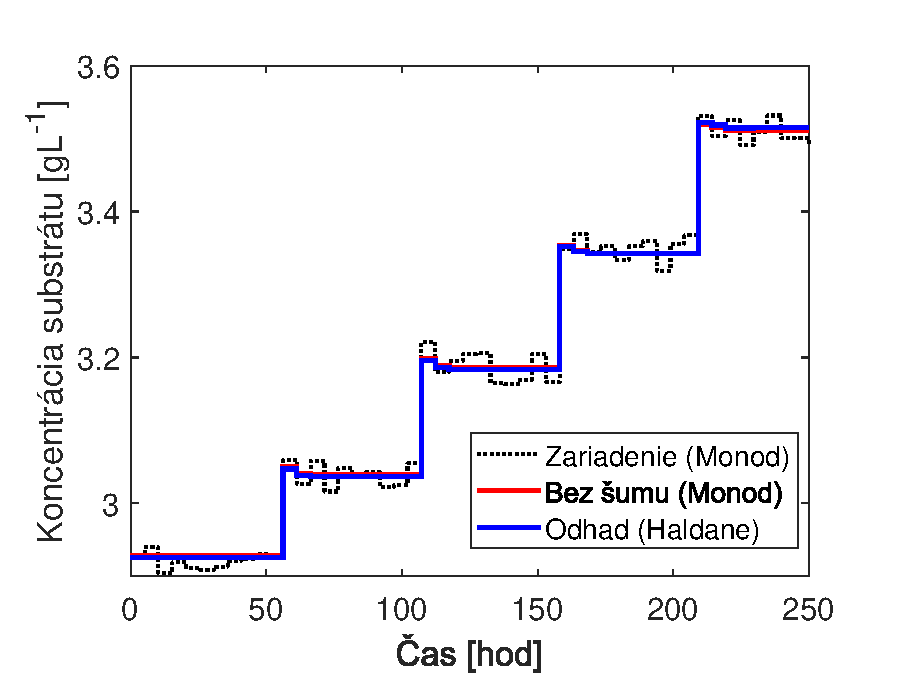
\includegraphics[width=\linewidth]{images/TwoStep_diff_sub}
		\caption{Odhad parametrov diferenciálnych rovníc.}
		\label{fig:twostep_diff_pe}
	\end{subfigure}
	\caption{Porovnanie prístupov k odhadu parametrov Haldane modelu na základe nameraných údajov zo zariadenia (Monod) pri viacerých skokových zmenách $ D=\lbrace D_{N}^{\star}, 0.38, 0.385, 0.39, 0.395 \rbrace \si{\per\hour} $.}
	\label{fig:twostep_pe_approach}
\end{figure}

Dvojkroková optimalizácia prebieha v dvoch fázach. Prvou je odhad parametrov nominálneho modelu na základe nameraných údajov zo zariadenia a v druhej fáze využívame tento model pri optimalizácii ustálených stavov zariadenia. Kvôli jasným výhodám, ktoré sme vyššie uviedli, budeme k odhadu parametrov pristupovať druhým spôsobom, teda tak ako uvádza rovnica \eqref{eq:twostep_diff_pe}.

Už Obr. \ref{fig:twostep_diff_pe} napovedal, že existuje kombinácia odhadovaných kinetických parametrov $ \mu_{m}, K_{M}, K{I} $ nominálneho modelu, ktorá dokáže simulovať naše zariadenie, a tým pádom vie predikovať správne hodnoty ustálených stavov. Tento fakt dokazuje aj Obr. \ref{fig:twostep_opt_costFun}. Na ňom vidíme priebeh hodnôt účelovej funkcie Monod modelu, teda reálneho zariadenia, počas jednotlivých iterácii. Ako môžeme sledovať, tak už v 5--6 iterácii dosiahne nominálny model optimálny stav zariadenia. Na ostatných obrázkoch \ref{fig:twostep_opt_muMax}, \ref{fig:twostep_opt_Km}, \ref{fig:twostep_opt_Ki} sú zobrazené hodnoty odhadnutých parametrov v jednotlivých iteráciách a bodkovane sú vyznačené parametre Monod modelu (v prípade maximálnej špecifickej rýchlosti rastu $ \mu_{m} $ a Michaelisovej konštanty $ K_{M} $), ale aj Haldane modelu, ktorým je určená začiatočná rýchlosť riedenia $ D_{N}^{\star} $. 

Nie je prekvapujúce, že iba na základe odhadu parametrov nepresného nominálneho modelu, sme dosiahli optimálnu prevádzku zariadenia. Je to spôsobené tým, že Monod aj Haldane modely sú si veľmi podobné. Jediný rozdiel medzi nimi je v špecifickej rýchlosti rastu $ \mu(s) $, kde Haldane model obsahuje v menovateli člen $ \frac{s^2}{K_{I}} $ navyše. Ak by sme limitne šli s inhibičným koeficientom do nekonečna $ K_{I} \rightarrow \infty $, zlomok $ \frac{s^2}{K_{I}} $ by šiel k nule $ \frac{s^2}{K_{I}} \rightarrow 0 $, a tým pádom by sme skonvergovali ku Monod modelu. Tento jav môžeme pozorovať na Obr. \ref{fig:twostep_opt_Ki}, kedy sa optimalizácia snaží vyrovnať rozdiely medzi modelmi, práve zväčšovaním hodnoty inhibičného koeficientu $ K_{I} $. Zvyšné dva parametre modelu konvergujú ku skutočným hodnotám zariadenia ako je ukázané na Obr. \ref{fig:twostep_opt_muMax} a \ref{fig:twostep_opt_Km}. 
\begin{figure}
	\centering
	\begin{subfigure}[b]{0.49\textwidth}
		\centering\
		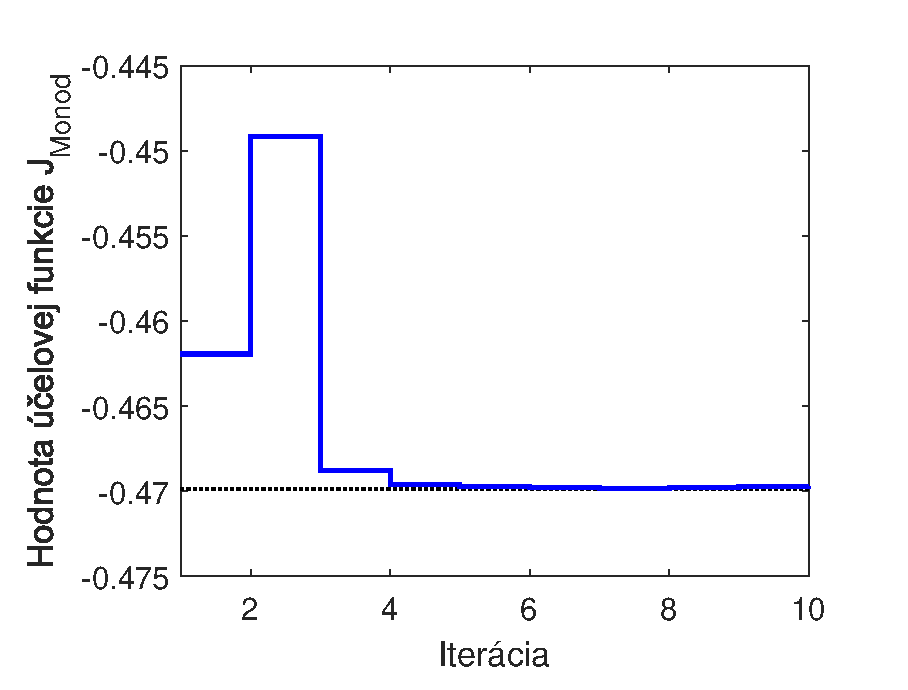
\includegraphics[width=\linewidth]{images/TwoStep_cost_fun}
		\caption{Optimá nominálneho modelu zobrazené ako hodnoty účelovej funkcie Monod modelu (zariadenia).}
		\label{fig:twostep_opt_costFun}
	\end{subfigure}
	\begin{subfigure}[b]{0.49\textwidth}
		\centering\
		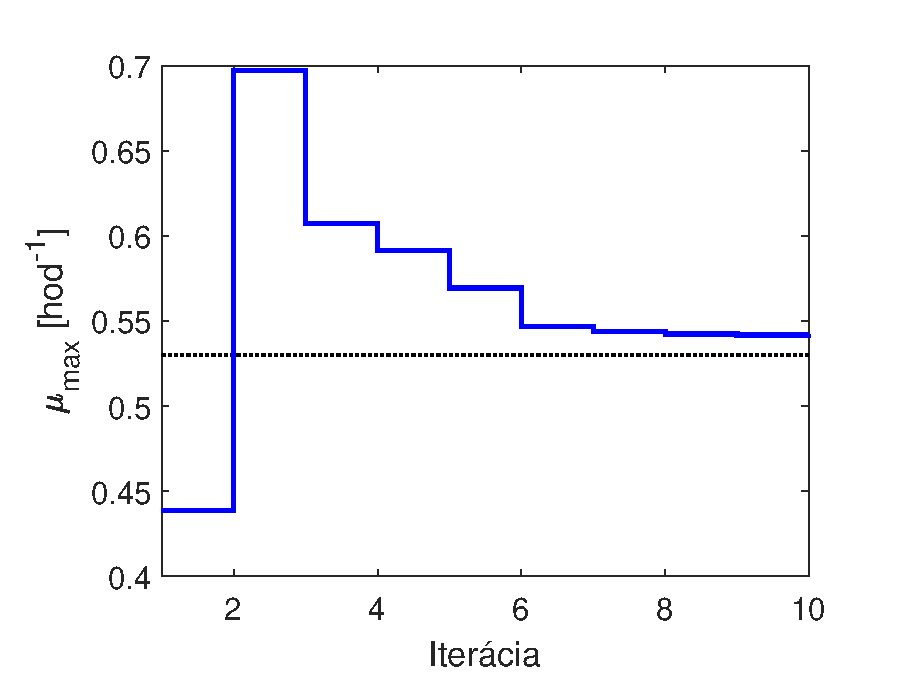
\includegraphics[width=\linewidth]{images/TwoStep_mu}
		\caption{Maximálna špecifická rýchlosť rastu. \newline \newline}
		\label{fig:twostep_opt_muMax}
	\end{subfigure}

	\bigskip

	\begin{subfigure}[b]{0.49\textwidth}
		\centering\
		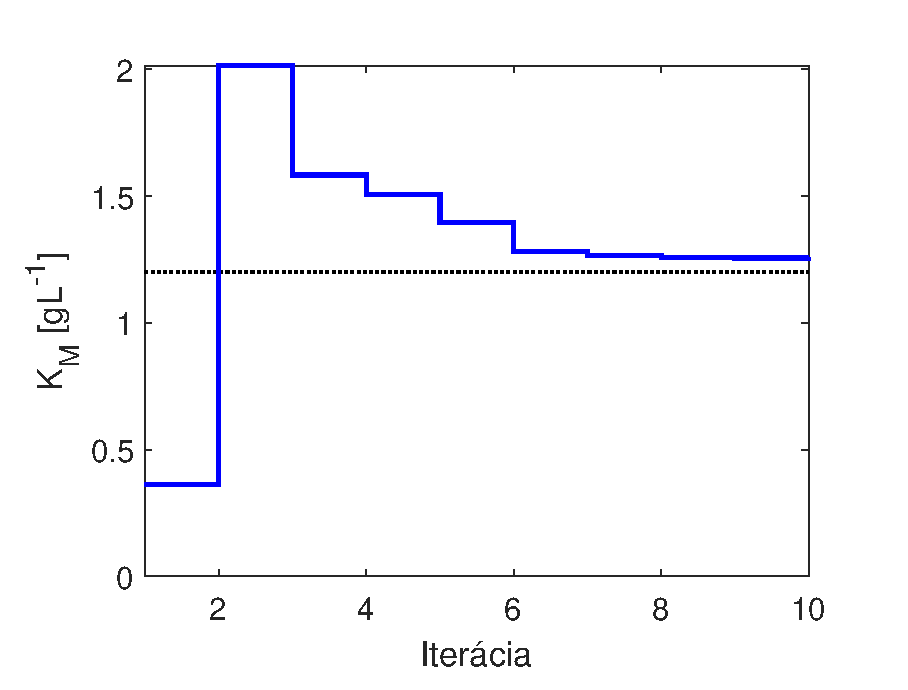
\includegraphics[width=\linewidth]{images/TwoStep_Km}
		\caption{Michaelisova konštanta.}
		\label{fig:twostep_opt_Km}
	\end{subfigure}
	\begin{subfigure}[b]{0.49\textwidth}
		\centering
		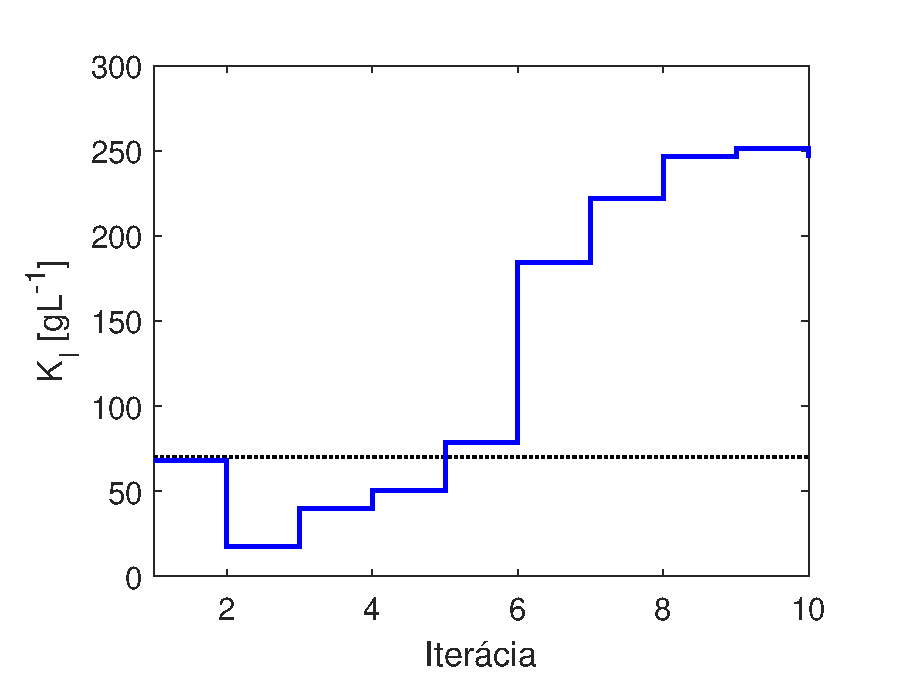
\includegraphics[width=\linewidth]{images/TwoStep_Ki}
		\caption{Koeficient inhibície.}
		\label{fig:twostep_opt_Ki}
	\end{subfigure}
	\caption{Priebeh optím Monod modelu vyjadrených ako hodnoty účelovej funkcie Monod modelu (zariadenia) a parametrov nominálneho modelu v jednotlivých iteráciach. Bodkovaná čiara znázorňuje hodnotu účelovej funkcie v optime zariadenia (a), alebo hodnoty parametrov pôvodného nastavenia nominálneho modelu (a, b, c) resp. zariadenia (b, c).}
	\label{fig:twostep_opt}
\end{figure}

Fakt, že modularita Haldane modelu a podobnosť oboch modelov nám umožnili skonvergovať ku skutočnému optimu zariadenia, je veľmi raritná a pri reálnych procesoch by takáto situácia teoreticky ani nenastala, pretože modelovanie zariadení so živými organizmami je komplikovaná záležitosť a výsledné modely majú zložitejšiu štruktúru ako Monod alebo Haldane model. 
